% document formatting
\documentclass[10pt]{article}
\usepackage[utf8]{inputenc}
\usepackage[left=1in,right=1in,top=1in,bottom=1in]{geometry}
\usepackage[T1]{fontenc}
\usepackage{xcolor}

% math symbols, etc.
\usepackage{amsmath, amsfonts, amssymb, amsthm}

% lists
\usepackage{enumerate}

% images
\usepackage{graphicx} % for images

% code blocks
\usepackage{minted, listings} 

% verbatim greek
\usepackage{alphabeta}

\graphicspath{{./assets/images/Week 1}}

\newcommand{\solution}{\textbf{Solution:}} 
\newcommand{\example}{\textbf{Example: }}
\newcommand{\water}{\text{H$_2$O}}
\newcommand{\hydroxide}{\text{OH$^-$}}
\newcommand{\hydronium}{\text{H$_3$O$^+$}}
\newcommand{\proton}{\text{H$^+$}}
\newcommand{\pc}{$^+$}
\newcommand{\nc}{$^-$}

\title{CHEM 153A Week 1}

\author{Aidan Jan}
\date{\today}

\begin{document}
\maketitle
\section*{Biochemistry}
\begin{itemize}
    \item It describes in molecular terms the structures, mechanisms, and chemical processes shared by all organisms and \textbf{provides organization principles} that underlie life in all its diverse forms.
\end{itemize}

\subsection*{How Molecular Processes Evolved}
\subsubsection*{The Great Oxidation Event (2.4-2.1B years ago)}
\begin{center}
\includegraphics*[width=\textwidth]{L1_1.png}
\end{center}
During this event, a few things happened:
\begin{itemize}
    \item Lots of species went extinct because of the change in atmosphere
    \item Animals can now exist, since aerobic respiration became possible
    \item Mitochondria began appearing.
\end{itemize}

\subsubsection*{Endosymbiotic Theory}
\begin{center}
    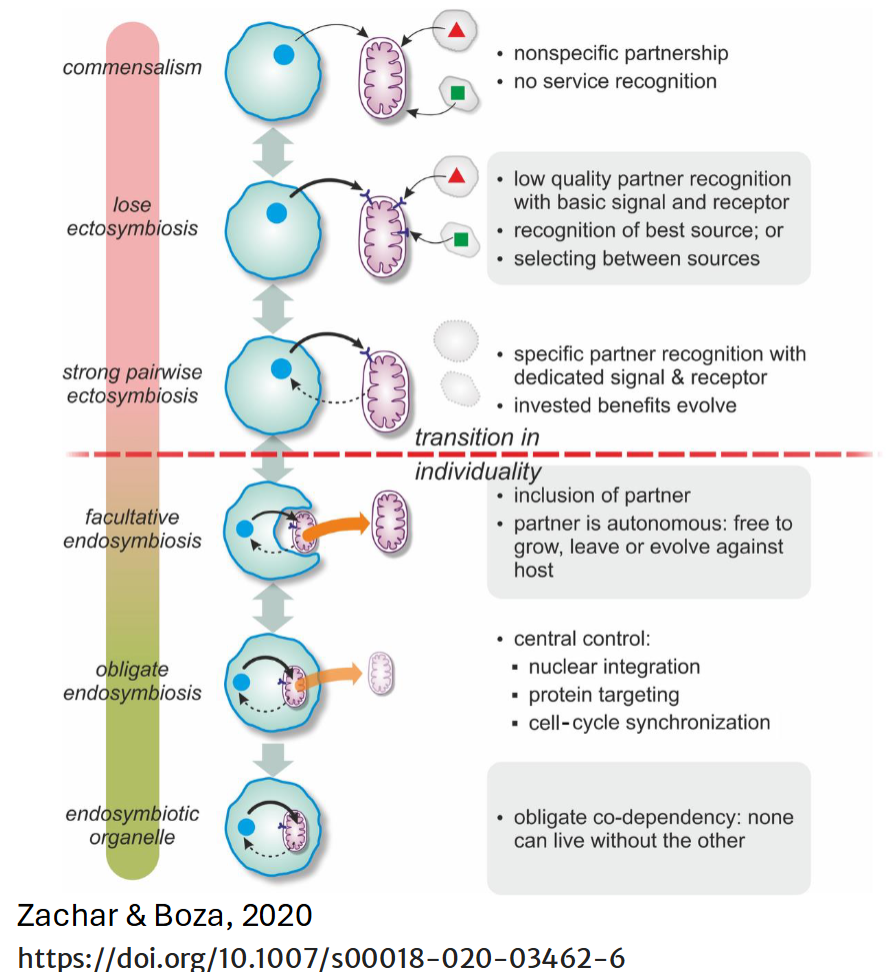
\includegraphics[scale=0.6]{L1_2.png}
\end{center}
\begin{itemize}
    \item Mitochondria used to be separate cells, rather than an organelle.
    \item At some point, one cell engulfed the other, and evolution occured.
\end{itemize}
\subsubsection*{Mitochondria}
\begin{center}
    \includegraphics*[scale=0.6]{L1_3.png}
\end{center}
\subsubsection*{Evolution of Metabolism}
\begin{itemize}
    \item This example alone demonstrates the transformative impact of oxygen in life
    \item \textbf{Biochemistry can be divided into two eras: one before oxygen, and one after}
    \item Modern processes depend on oxygen, while older, more ancient pathways functioned in its absence.
\end{itemize}
\begin{center}
    \includegraphics*[width=\textwidth]{L1_4.png}
\end{center}
\subsubsection*{Proteins}
\begin{center}
    \includegraphics*[width=\textwidth]{L1_5.png}
\end{center}
\begin{itemize}
    \item The above diagram shows proteins, an important part of cells and metabolism.
    \item This class aims to study the metabolic pathways in cells, many of which are catalyzed by proteins (specifically enzymes).
    \item RNA can also be a catalyst.  (RNA is not a protein)
\end{itemize}
\section*{Water}
\begin{center}
    \includegraphics*[width=\textwidth]{L1_6.png}
\end{center}
\begin{itemize}
    \item Water is a dominant metabolite in biochemistry, accounting for 99.4\% by molarity of metabolites within an \textit{E. coli.} bacteria.  Water in an \textit{E. coli} cell is around 40 M.  The sum of the concentrations of all other metabolites is 240 mM.
\end{itemize}
\subsection*{Proteins Exist in Aqueous Environments}
\begin{itemize}
    \item Our first major topic in this class is \textbf{protein synthesis and structure}
    \begin{itemize}
        \item The \textbf{amino acids} of proteins are affected by the \textbf{pH} of aqueous environments (protonation state!)
        \item These amino acids often form different \textbf{intermolecular interactions} amongst themselves and with their environment
        \item The folding of proteins is a \textbf{thermodynamic} problem
    \end{itemize}
\end{itemize}
\subsection*{Importance of Water}
\begin{itemize}
    \item Physical and chemical properties of water influence every biochemical interaction
    \begin{itemize}
        \item The medium for most biochemical reactions
        \item Participates directly in many biochemical reactions
        \item Affects folding (structure) of biomolecules
    \end{itemize}
\end{itemize}
\subsubsection*{Aside: Quantifying the amount of substance dissolved in a solvent}
\begin{itemize}
    \item Concentration measures how much \textbf{solute} (the substance being dissolved) is present in a certain volume of \textbf{solvent} (usually water)
    \item Use Molarity (M).
    \begin{itemize}
        \item Definition: Moles of solute per liter of solution
        \item Formula: $M = \frac{\text{Moles solute}}{\text{Liters solution}}$
        \item Example: A 1M NaCl solution contains 1 mole of NaCl in 1 liter of water.
        \item Square brackets are used in chemistry to represent the concentration of a substance.
    \end{itemize}
\end{itemize}
\subsection*{Our Watery Origins}
\subsubsection*{Water as Essential but Problematic}
\begin{itemize}
    \item \textbf{Essential for Life:} Water is crucial for life because it acts as a solvent, facilitates biochemical reactions, and is involved in virtually all life processes
    \item \textbf{Problematic for Life's Origins:} Paradoxically, water can hinder the formation of important biomolecules, such as proteins and nucleic acids, because both are \textbf{condensation polymers}.  This means that their formation involves reactions that produce water as a byproduct.  In an aqueous environment, water tends to promote the reverse reaction, hydrolysis, which breaks down these polymers
    \item The key to overcoming this challenge lies in \textbf{balancing thermodynamic activation} (making the formation of polymers energetically favorable) with \textbf{kinetic stability} (preventing them from breaking down too easily)
\end{itemize}
\begin{center}
\fbox{
    \parbox{0.9\textwidth}{
        \textbf{Prebiotic chemistry} could bypass fully hydrolyzed monomers and use energy-rich intermediates for polymer formation\\\\
        Example: \textbf{ATP}, though thermodynamically unstable in water, remains kinetically stable enough to drive biochemical reactions
    }
} 
\end{center}
\begin{itemize}
    \item Liquid water is an extraordinary molecule that plays a central role in the chemistry of life due to its unique properties.
    \item The most important among them probably are the ability to establish hydrogen bonds, a high polarity and a high dielectric constant
\end{itemize}
\subsubsection*{Kinetic vs. Thermodynamic Stability}
\begin{itemize}
    \item \textbf{Thermodynamic Stability:} Determines \underline{whether a reaction will be energetically favorable, or spontaneous}, based on the overall energy of the system.  A thermodynamically stable molecule is one that is in a lower energy state compared to its potential products
    \item \textbf{Kinetic Stability:} Refers to how \underline{quickly (or slowly) a reaction proceeds}.  A kinetically stable molecule is one that reacts very slowly, even if the reaction would be favorable (thermodynamically stable).
\end{itemize}
\begin{center}
    \includegraphics*[width=\textwidth]{L2_1.png}
\end{center}
\subsection*{Hydrogen Bonds}
\begin{itemize}
    \item Hydrogen bonds are crucial for the unique properties of water, enabling its role as a solvent and in biochemical reactions.
    \item Water molecules can form hydrogen bonds because of the polarity in their O-H bonds.  Oxygen, being more electronegative, pulls shared electrons closer, creating a partial negative charge on the oxygen and partial positive charges on the hydrogen atoms
    \item This polarity allows water to generate a cohesive hydrogen-bond network, resulting in phenomena such as high surface tension and capillary action, and enabling it to dissolve many polar substances effectively.  Hydrogen bonding also stabilizes biological macromolecules (e.g., proteins, nucleic acids)
    \item Water has a higher melting point, boiling point, and heat of vaporization than most other common solvents (due to polarity and H-bonds)
    \item Hydrogen bond (H-bond) = \textbf{electrostatic attraction between the oxygen atom of one water molecule and the hydrogen of another}
\end{itemize}
\begin{center}
    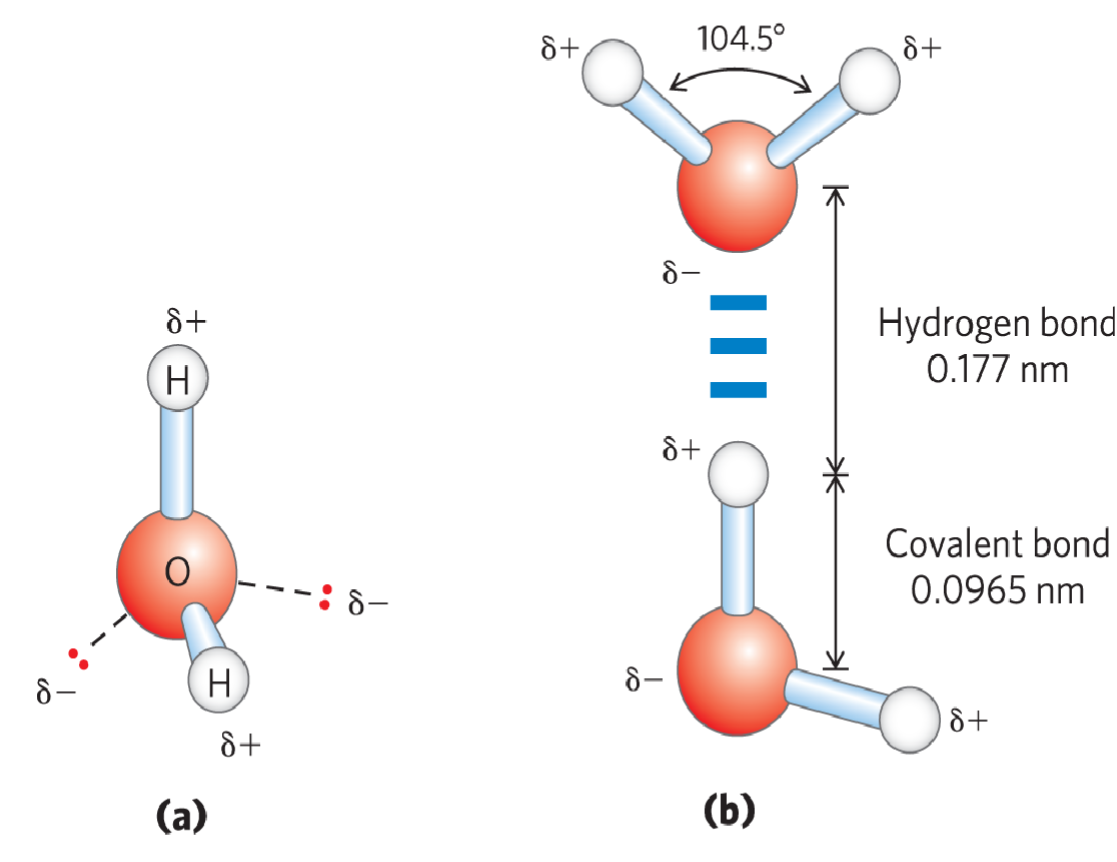
\includegraphics[scale=0.5]{L2_2.png}
\end{center}
\subsubsection*{Strength of Hydrogen Bonds}
\begin{itemize}
    \item Hydrogen bonds are \textbf{relatively weak}
    \begin{itemize}
        \item bond dissociation energy (energy req  uired to break a bond) = ~23 kJ/mol in liquid H$_2$O (~470 kJ/mol for a covalent O-H bond)
        \item 1\% covalent, 90\% electrostatic
    \end{itemize}
    \item Hydrogen bonds are fleeting
    \begin{itemize}
        \item lifetime of each hydrogen bond is just 1 to 20 picoseconds in liquid (1 picosecond = $10^{-12}$ seconds)
        \item when one hydrogen bond breaks, another forms
    \end{itemize}
\end{itemize}
\subsubsection*{Number of Hydrogen Bonds Formed}
\begin{itemize}
    \item In liquid, each H$_2$O molecule forms hydrogen bonds with an average of 3.4 other molecules
    \item In ice, each H$_2$O molecule forms 4 hydrogen bonds.
\end{itemize}
\subsubsection*{Water and Polar Solutes}
\begin{itemize}
    \item Hydrogen bonds form between:
    \begin{itemize}
        \item Hydrogen acceptor: Electronegavie atom (e.g., O or N)
        \item Hydrogen donor: H covalently bonded to another electronegative atom
    \end{itemize}
    \item Important note: H atoms bonded to carbon do not participate in hydrogen bonding
\end{itemize}
\subsection*{Acids and Bases and Water}
\begin{itemize}
    \item The concept of acids and bases is entirely mediated by water.
\end{itemize}
\begin{center}
    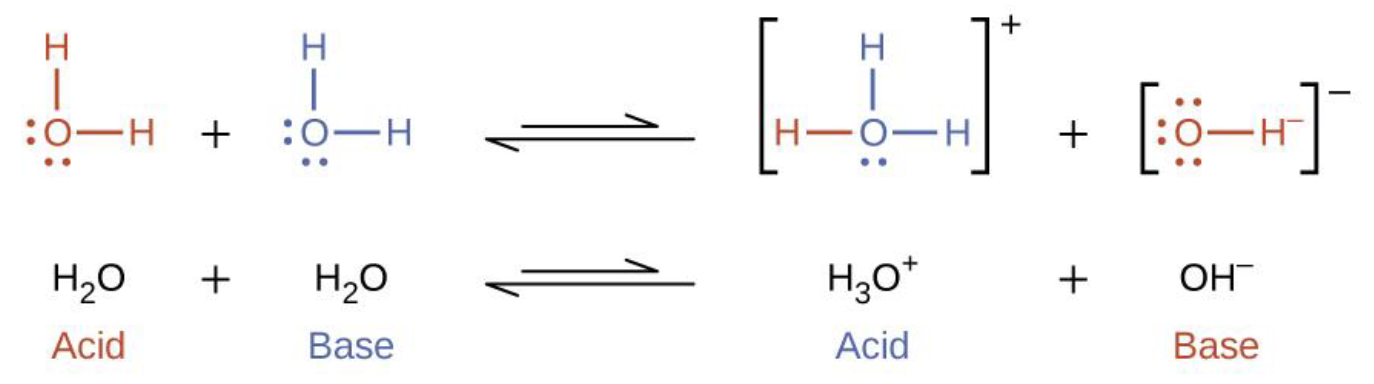
\includegraphics[width=\textwidth]{L3_1.png}
\end{center}
\fbox{
    \parbox{\textwidth}{
        The \textbf{autoionization of water} is the process by which two water
        molecules interact to form a hydronium ion (H$_3$O$^+$) and a hydroxide
        ion (OH$^-$). This occurs even in pure water, albeit at a very low rate,
        leading to an equilibrium concentration of H$_3$O$^+$ and OH$^-$ ($10^{-7}$ M
        each at 25$^\circ$C, corresponding to a neutral pH of 7)
    }
} 
\subsection*{Acids and Bases: Brønsted-Lowry Definitions}
\begin{itemize}
    \item \textbf{Acids} are \textbf{proton donors}
    \item \textbf{Bases} are \textbf{proton acceptors}
    \item \textbf{Acid-base reactions} are \textbf{proton transfers}
\end{itemize}
Many reactions that occur in nature are \textbf{\textit{\underline{reversible}}} and do not proceed to completion.
Instead, they come to an apparent halt or \textbf{\textit{\underline{equilibrium}}} at some point between 0 and 100\% completion.
\textbf{\textit{\underline{At equilibrium, the net}}} \textbf{\textit{\underline{velocity is zero}}} because the absolute velocity in the forward direction exactly
equals the absolute velocity in the reverse direction.
The position of equilibrium is conveniently described by an equilibrium constant, K$_{\text{eq}}$.
For example, consider the dissociation of a weak acid:
\subsection*{Ionization Constants}
\begin{itemize}
    \item the tendency for any acid (HA) to lose a proton and form
    its conjugate base (A$^-$) is defined by the equilibrium
    constant (K$_{\text{eq}}$) for the reversible reaction
\end{itemize}
\begin{center}
HA $\rightleftharpoons$ H$^+$ + A$^-$
\end{center}
for which
\[K_{eq} = \frac{\text{[H\pc][A\nc]}}{[\text{HA}]} = K_a\]
The acid dissociation constant ($K_a$) is a measure of the extent to which an acid dissociates in solution and therefore its \textbf{\underline{strength}}.  The less an acid dissociates, the smaller the value of $K_a$.  The stronger the acid, the higher the value of $K_a$.\\\\
The ionization behavior of water and of weak acids and bases dissolved in water can be represented by one or more equilibrium constants.
Most biomolecules are ionizable; their structure and function depend on their ionization state, which is characterized by equilibrium constants.\\\\
In general:
\[K = \frac{\text{[P]}}{\text{[R]}}\]
\[aA + bB \rightleftharpoons cC + dD\]
\subsubsection*{The Ion Product of Water}
\[K_w = K_{\text{\water}} = \text{[H$_3$O$^+$][OH$^-$]} = 1 \times 10^{-14} \text{M}^2\]
As a consequence, neutral pH = exactly equal concentrations of H\pc and OH\nc as in pure water.\\\\
At neutral pH:
\begin{align*}
K_w &= \text{[H$^+$][OH$^-$]} = \text{[H$^+$]}^2 = \text{[OH$^-$]}^2\\
\text{[H$^+$]} &= \sqrt{K_w} = \sqrt{1.0 \times 10^{-14} \text{ M}^2}\\
\text{[H$^+$]} &= \text{[OH$^-$]} = 10^{-7} \text{M}
\end{align*}
\subsection*{The pH Scale Designates the H\pc and OH\nc Concentrations}
\begin{itemize}
    \item the pH scale is based on the ion product of water, $K_w$
    \item the term pH is defined by the expresson:
    \[\text{pH} = \log\frac{1}{\text{[H$^+$]}} = -\log \text{[H$^+$]}\]
    where
    [H$^+$] = [OH$^-$] = $10^{-7}$ M
    \item for a precisely neutral solution at 25$^\circ$C, pH = 7.0
\end{itemize}
\subsection*{The Mechanism of Autoionization}
\begin{center}
    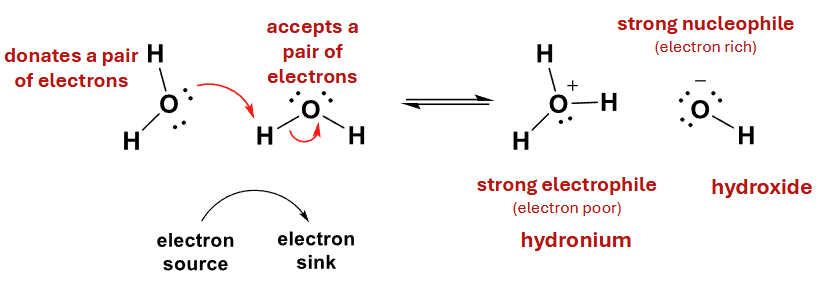
\includegraphics[width=\textwidth]{L3_2.png}
\end{center}
\subsection*{Lewis Acids and Lewis Bases}
\begin{itemize}
    \item \textbf{Lewis base} - Any molecule (or ion) that can form a new covalent bond by \underline{donating a pair of electrons}
    \begin{itemize}
        \item Also called a \textbf{nucleophile} ("nucleus loving")
        \item Electron rich (-, $\delta^-$, lone pairs, pi-bonds)
        \item \underline{Examples:} \water, \hydroxide, H$_2$C$=$CH$_2$
    \end{itemize}
    \item \textbf{Lewis acid} - Any molecule (or ion) that can form a new covalent bond by \underline{accepting a pair of electrons}
    \begin{itemize}
        \item Also called an \textbf{electrophile} ("electron loving")
        \item Electron poor (+, $\delta^+$, unfilled octet)
        \item \underline{Examples:} \hydronium, \pc CH$_3$, H$_3$C$-$Cl
    \end{itemize}
\end{itemize}
\begin{center}
    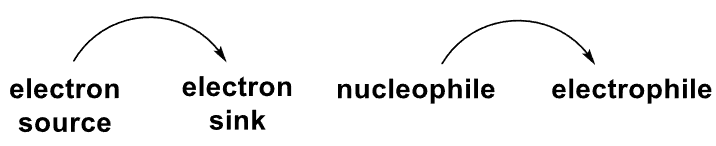
\includegraphics[scale=0.5]{L3_3.png}
\end{center}
\subsection*{The pH of Some Aqueous Fluids}
\begin{itemize}
    \item pH values > 7:
    \begin{itemize}
        \item alkaline or basic
        \item concentration of \hydroxide is greater than that of \proton
    \end{itemize}
    \item pH values < 7:
    \begin{itemize}
        \item acidic
        \item concentration of \proton is greater than that of \hydroxide
    \end{itemize}
\end{itemize}
\begin{center}
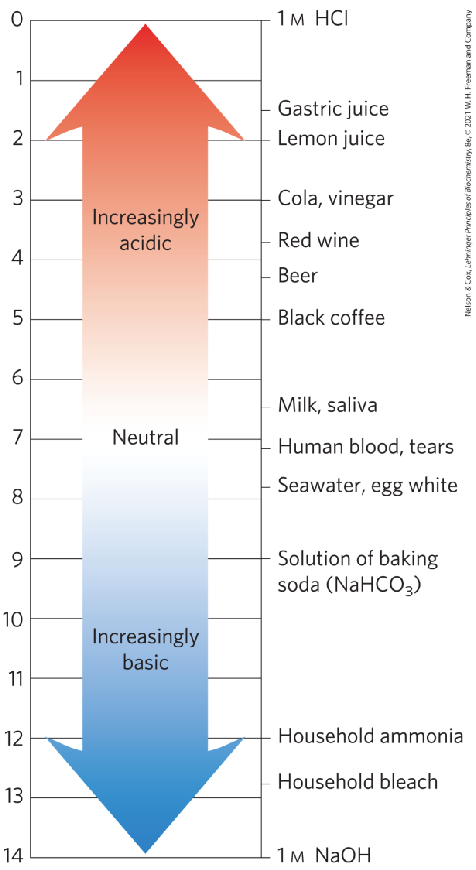
\includegraphics[scale=0.5]{L3_4.png}
\end{center}
\subsection*{pH and Medical Diagnoses}
\begin{itemize}
    \item acidosis = pH of blood plasma below the normal value of 7.4
    \begin{itemize}
        \item common in people with severe, uncontrolled diabetes
    \end{itemize}
    \item alkalosis = pH of blood plasma above the normal value of 7.4
    \item extreme acidosis or alkalosis can be life-threatening
\end{itemize}
\subsection*{Conjugate Acid-Base Pairs}
\begin{itemize}
    \item conjugate acid-base pair = a proton donor and its corresponding proton acceptor
    \item the stronger the acid, the greater its tendency to lose its proton
\end{itemize}
\begin{center}
    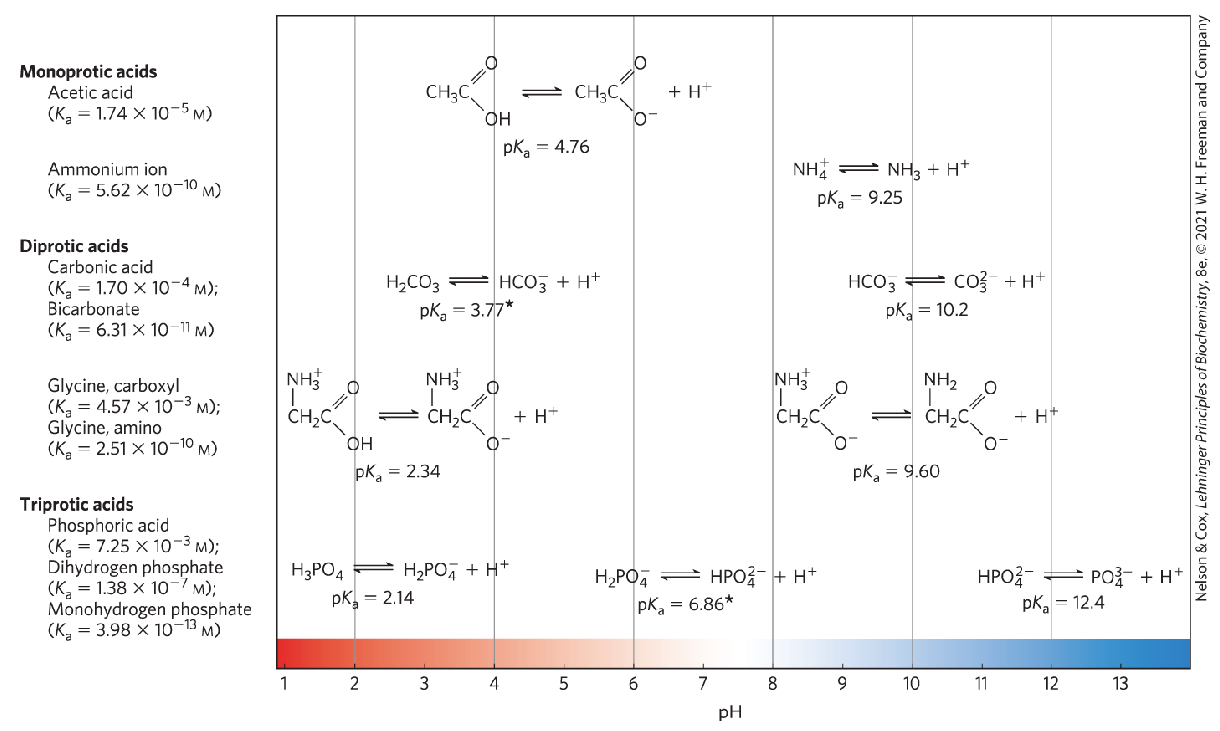
\includegraphics[width=\textwidth]{L3_5.png}
\end{center}
\subsection*{p$K_a$}
\begin{itemize}
    \item p$K_a$ = analogous to pH and defined by the equation
    \[\text{p}K_a = \log\frac{1}{K_a} = -\log K_a\]
    \item the stronger the tendency to dissociate a proton, the \underline{\textbf{stronger the acid} and \textbf{the lower its p$K_a$}}
    \item p$K_a$ can be determined experimentally
\end{itemize}




\end{document}
